
\subsection{Теоретико-ігрова інтерпретація моделі Барро-Гордона}

У грі беруть участь два гравці: $p$ - уряд, $q$ - громадськість, які оперують інфляцією $\pi$ і індексуванням заробітної плати $\omega$ відповідно. Для спрощення моделі покладемо, що обидва не можуть прогнозувати майбутнє. Кожен гравець вибирає з наступних стратегій: низьким $L$ і високим  $H$ рівнем підвищення. У загальному вигляді гра може бути задана у вигляді матриці виграшів,
\begin{table}[h]
	\centering
	\caption{}
 Матриця виграшів в моделі Барро-Гордона\\
\normalsize
\begin{tabular}{|l|l|c|c|}
	\hline
	\multicolumn{2}{|l|}{\multirow{2}{*}{}} & \multicolumn{2}{l|}{Громадськість} \\ \cline{3-4} 
	\multicolumn{2}{|l|}{}                  & L                & H                \\ \hline
	\multirow{2}{*}{Уряд}    & L   & a,q              & b,v              \\ \cline{2-4} 
	& H   & c,x              & d,z              \\ \hline
\end{tabular}
\end{table}\\
де параметри $a,b,c,d,q,v,x,z$  - виграші задовольняючi наступним обмеженням~\cite{libich2008macroeconomic}

\begin{equation}
c>a>d>b, q>v, q\geqslant z>x.
\label{eq:sec:ot:restrictions}
\end{equation}

В даному випадку найпростіше описати економіку через функцію сукупної пропозиції Лукаса~\cite{libichIncorpo}

\begin{equation}
\label{eq:sec:ot:lucas}
y_t - Y = \lambda(\pi_t - \omega_t)+\varepsilon_t,
\end{equation}
де  $\lambda>0, y$  – продуктивність, $Y$ – природний рівень продуктивності, а $\varepsilon$ - макроекономічний шок близький до нуля. Коефіцієнти дисконтування гравців складають $\beta_g$ и $\beta_p$, а їх функції корисності мають наступний вигляд

\begin{equation}
\label{eq:sec:ot:govUtil}
u^g_t=-(\pi_t - \tilde{\pi})^2 + \alpha y_t - \beta(y_t-Y)^2,
\end{equation}

\begin{equation}
\label{eq:sec:ot:pubUtil}
u^p_t=-(\pi_t - \omega)^2,
\end{equation}
де $\tilde{\pi}$ - оптимальний рівень інфляції, а $\alpha > 0, \beta > 0$ описують відносну вагу цілей уряду (стабільної інфляції, високої і стабільної продуктивності). Громадськість стурбована вірним очікуванням рівня інфляції для того, щоб визначити рівень зарплат на ринку.
\\

Так як нас цікавить ефект від обраної політики, то сфокусуємось на довгостроковому результаті гри. Для цього однозначно визначимо економіку поклавши $\forall t$,      $\varepsilon_t=0$ , що передбачає, що ми можемо покласти $\beta=0$ без втрати спільності. З цього випливає, що інструмент уряду $\pi$  є вибір середньої інфляції.
\\

У стандартній покрокової грі, в якій гравці можуть змінювати свою поведінку в кожен період, ми використовуємо \eqref{eq:sec:ot:lucas}-\eqref{eq:sec:ot:govUtil} для отримання рівноваги
\begin{equation}
\label{eq:sec:ot:equilibrium}
\pi^*_t= \tilde{\pi} + \frac{\alpha\lambda}{2}= \omega^*_t,
\end{equation}
що є відомим результатом  $\pi^*_t > \tilde{\pi}$. Сфокусувавши увагу на двох рівнях інфляції ми слідуємо ~\cite{ChoiAndMacui96InflationFinancialMarkets}, де були запропоновані два найбільш природних варіанти - оптимальний рівень з \eqref{eq:sec:ot:govUtil} і узгодженого по часу з \eqref{eq:sec:ot:equilibrium}

\begin{equation}
\label{eq:sec:ot:optimal}
\pi \in \left\{L=\tilde{\pi}, H=\tilde{\pi}+\frac{\alpha\lambda}{2} \right\} \ni \omega^*_t.
\end{equation}

Ми можемо, враховуючи \eqref{eq:sec:ot:lucas}-\eqref{eq:sec:ot:pubUtil}і поділивши на $\left(\frac{\alpha\lambda}{2}\right)$,  без втрати спільності вивести відповідні виграші, представлені в таблиці нижче. Так само незалежно від $\lambda$ та  $\alpha$ справедливі такі обмеження для даної гри на додаток до початкових~(\ref{eq:sec:ot:restrictions})

\begin{equation}
	\label{eq:sec:ot:constraint}
	c>a=0 > d > b,c=-d=-\frac{b}{2}, q>v,q\geqslant z>x
\end{equation}

\begin{equation}
\label{eq:sec:ot:exampleConstraint}
c=1 > a=0 > d=-1 > b=-2, q=z=0 > v=x=-1,
\end{equation}

\begin{table}[h]
	\centering
	
	\caption{}	
 Матриця виграшів з~(\ref{eq:sec:ot:exampleConstraint})\\
	\normalsize
\begin{tabular}{|l|l|c|c|}
	\hline
	\multicolumn{2}{|l|}{\multirow{2}{*}{}} & \multicolumn{2}{l|}{Громадськість} \\ \cline{3-4} 
	\multicolumn{2}{|l|}{}                  & L                & H                \\ \hline
	\multirow{2}{*}{Уряд}    & L   & 0, 0             & -1,-1            \\ \cline{2-4} 
	& H   & $\frac{1}{2}$,-1             & $-\frac{1}{2}$, 0            \\ \hline
\end{tabular}
		
	\label{table:sec:ot:real}
\end{table}


Стандартна покрокова гра має унікальну рівновагу Неша$(H,H)$. Однак, воно неефективно, так як є Парето домінуючим. Це означає, що існує такий результат гри, який поліпшить стан одного, але при цьому не погіршить його для інших гравців. В даному випадку це «не Нешовскій» результат $(L,L)$.  В уряду виникає спокуса створити несподівану інфляцію, щоб підвищити продуктивність і знизити рівень безробіття. Так як громадськість раціональна, то буде чекати високу інфляцію - обидва гравці будуть в програші.

\subsection{Стійкість рівноважних стратегій в моделі Барро-Гордона на
	часових шкалах} 

Розглянемо ігрову інтерпретацію моделі Барро-Гордона на часових шкалах.

Усі припущення висунуті в стандартній грі залишаються. Розширимо їх:
\begin{itemize}
	\item гра починається одночасним ходом, 
	\item заздалегідь відомо незмінне кількість ходів $r^g \in \mathbb{N}$ та $r^p \in \mathbb{N}$,
	\item гра закінчується через $T$ періодів, де $T$ - найменше спільне кратне для $r^g$ та $r^p$,
	\item гравці раціональні, мають рівноцінними знаннями і повною інформацією про структуру гри, матриці виграшів і всіх попередніх ходах.
\end{itemize}

Іншими словами визначається три часові шкали: уряду, громадськості та самої гри:
\begin{equation}
\label{eq:sec:tech:scales}
T_g = \{0,r^g,2r^g,...,T\}, T_p=\{0,r^p,2r^p,...,T\}, T=T_g\cup T_p 
\end{equation}

Головною перевагою використання однорідних часових шкал є економічна інтерпретація: $r^g$ та $r^p$ являють собою ступінь можливості змін політики щодо інфляції і ступінь реагування для внесення змін до заробітні плати.
\\

Асинхронна гра на часових шкалах буде як правило мати кілька рівноваг Неша, серед яких ми виберемо найкращу в залежності від під-гри.

\begin{theorem}
Розглянемо загальну неузгоджену по часу гру на однорідних часових шкалах, для якої виконуються ~(\ref{eq:sec:ot:constraint}) та ~(\ref{eq:sec:tech:scales}). Тоді все SNPE гри будуть SNPE Рамсея, якщо і тільки якщо
	
	\begin{equation}
	\label{eq:sec:tech:theoremSystem}
	r^g> \bar{r^g}(R) = \left\{ 
	\begin{aligned} 
	&\frac{c - d}{a-d}r^p= \frac{a-b}{a-d}r^p, &&\text{якщо } R=0
	\\
	&\frac{(1+R)(c-d)}{a-d}r^p= \frac{a-b + R(c-d)}{a-d}r^p, &&\text{якщо } 	R\in(0; \bar{R})
	\\
	&\frac{c-d-(1-R)(a-b)}{a-d}r^p= \frac{(a-b)}{a-d}Rr^p, &&\text{якщо } 	R\in(\bar{R};1)
	\end{aligned}
	\right.		
	\end{equation}
\end{theorem}
де $\bar{R}=\frac{q-v}{z-x+q-v}$. У неузгодженiй грі, де справедливо ~(\ref{eq:sec:ot:constraint}),  ~(\ref{eq:sec:tech:theoremSystem}) перетвориться в

\begin{equation}
\frac{r^g}{r^p} \in \left(\frac{3}{2}, 2\right)\cup \left(\frac{5}{2}, \infty\right)
\end{equation}
Доказ: дивитися Либиха і Штелиха~\cite{libichIncorpo}.


Можна стверджувати, що дії гравців можуть не завжди бути детерминистическими і / або що частота їх ходів різниться в часі або підпорядковується деякому випадковому процесу. Різнорідні тимчасові шкали дозволяють вивчати подібні випадки. Для більшої ефективності нормалізуємо горизонт планування як $T = r^g$. Як і раніше гравці $g$ та $p$ ходять одночасно в першому періоді і в усіх $T = r^g$ періодах, в проміжках між якими громадськість так само здатна реагувати на хід уряду. Для зручності порівняння залишимо всі припущення попереднього параграфа незмінними.

Розглянемо довільну тимчасову шкалу $\mathbb{T}$ і довільну незростаючу функцію реакції громадськості $f : \mathbb{T} \to [0,1]$. У даній роботі розглядаються два становлячих інтерес особливих випадки. У першому, при різноріднiй (атомістичної) громадськості, функція реакції може бути інтерпретована як частина громадськості, яка вже мала можливість зробити хід. У другому, при ймовірних ходах громадськості, функція реакції може бути інтерпретована як кумулятивна функція розподілу її ходів.

Щоб упевнитися в тому, що всі SPNE є SPNE Рамсея, досить показати, що в першому ході оптимальною стратегією $g$ є $L$ незалежно від ходу громадськості в першому періоді. Отримаємо два відповідних умови:
\begin{equation}
\label{sec:hetero:main1}
ar^g > c \int_0^{r^g} 1 - f(t) \Delta t + d  \int_0^{r^g} f(t) \Delta t ,
\end{equation}
\begin{equation}
\label{sec:hetero:main2}
dr^g > b \int_0^{r^g} 1 - f(t) \Delta t + a  \int_0^{r^g} f(t) \Delta t .
\end{equation}

\begin{theorem}
	\label{spneTh}
Розглянемо загальну неузгоджену по часу гру, в якій виконується~\eqref{eq:sec:ot:constraint} та $f : \mathbb{T} \to [0,1]$ -- незростаюча функція реакції. Тоді все SPNE гри є SPNE Рамсея тоді і тільки тоді, коли виконується нерівність
	\begin{equation}
	\label{sec:hetero:main3}
	\int_0^{r^g} f(t) \Delta t > \frac{r^g}{2} .
	\end{equation}
\end{theorem}

Для кращої наочності теореми~\ref{spneTh} і кращого розуміння наведемо кілька наслідків і розглянемо приклад. Як вже було зазначено раніше, ми концентруємося на двох випадках: різноріднiй громадськості та ймовірних моделях.

\subsubsection{Різнорідна громадськість.} По-перше, припустимо, що існує $ N $ різних громадських груп (профспілок) $p_1,...,p_N$ з відповідними  $r^{p_1},...,r^{p_N}$ і розмірами $s_1,...,s_N \in [0,1]$, які задовольняють природним припущенням  $\sum_{i=1}{N}s_i = 1$. Щоб звести нашу увагу до першого ходу уряду, припустимо що $r^g$ є кратним для $r^{p_i}$ для всіх $i = 1,...,N$, тобто
$$ \frac{r^g}{r^{p_i}} \in \mathbb{N}.$$
Для більш асинхронних випадків див.~\cite{libichIncorpo}. Для даного особливого випадку теорему~\ref{spneTh} можна переписати наступним чином.\\
\textbf{Наслідок 1.} \textit{Розглянемо загальну неузгоджену по часу гру, в якій виконується~\eqref{eq:sec:ot:constraint}і громадськість складається з $ N $ різних груп. Тоді все SPNE гри є SPNE Рамсея тоді і тільки тоді, коли виконується нерівність
	\begin{equation}
	\label{sec:hetero:main4}
	\sum_{i=1}^N s_i(r^g - r^{p_i}) \geqslant \frac{r^g}{2} .
	\end{equation}
}
%опять же доказательство

\subsubsection{Імовірнісна модель.}
Повернемося до випадку з уніфікованою громадськістю, щоб розглянути ймовірні ходи окремо від впливу ефектів різнорідної громадськості. Залежно від результатів переговорів громадськість реагуватиме на перший хід уряду в якийсь момент часу з інтервалу  $[a,b], 0< a < b < r^g$, з рівномірно розподіленим імовірнісним законом. Теорема~\ref{spneTh} набирає вигляду:\\
\textbf{Наслідок 2.} \textit{Розглянемо загальну неузгоджену по часу гру, в якій виконується~\eqref{eq:sec:ot:constraint} і громадськість робить другий хід в якийсь момент часу з інтервалу $[a,b]$ з рівномірно розподіленим імовірнісним законом. Тоді все SPNE гри є SPNE Рамсея тоді і тільки тоді, коли виконується нерівність
	\begin{equation}
	\label{sec:hetero:main5}
	\frac{b^2 - a^2}{2} \geqslant b - \frac{r^g}{2} .
	\end{equation}
}
Зрозуміло, що можна розглядати довільні комбінації описаних вище підходів, тобто різнорідних гравців з ймовірними ходами, ймовірність яких може бути описана деякими функціями розподілу. Наведемо приклад.\\
\textbf{Приклад 1.} Розглянемо економіку з двома профспілками, кожна з яких складається з $s_1$ та $s_2$ робітників відповідно, так що виконується $s_1 + s_2 = 1$. Приймемо в якості одного періоду квартал (раз в квартал випускаються зведення з макроекономіки). Припустимо, що $r^g = 5$ і що час реакції профспілок складають як мінімум 1 і 3 квартали, але як максимум - 1,5 і 3,5 квартали відповідно. Для простоти припустимо, що рішення, прийняте за півтора кварталу підпорядковується рівномірному закону розподілу. Тоді отримаємо:
$$ \mathbb{T} :={0} \cup [1, 1.5] \cup {r^g} ,$$
$$ \mathbb{T} :={0} \cup [3, 3.5] \cup {r^g} .$$
Функція реакції тоді має вигляд$f : \mathbb{T}_1\cup\mathbb{T}_2\to[0,1]$:
$$ f(x)\left\{  
\begin{array}{l c l}
0 & if & x = 0,\\
2s_1(x - 1) & if & x \in [1,1.5],\\
s_1 + 2s_2(x - 3) & if & x \in [3,3.5],\\
1 & if & x = 5.
\end{array} 
\right.$$
Iнтегруючи по $\mathbb{T}_1\cup\mathbb{T}_2$ отримаємо
$$ \int_0^5 f(x) \Delta x = \frac{15}{4}s_1 + \frac{7}{4}s_2. $$
Припущення~\eqref{sec:hetero:main3} теореми~\ref{spneTh} задовольняється (і отже єдиною рівновагою є рівновага Рамсея) тоді і тільки тоді, коли виконується
$$ s_1 \geqslant \frac{3}{8}, \text{або, що еквівалентно,} s_2 \leqslant \frac{5}{8}. $$
Інтуїтивно зрозуміло, що профспілка, яка приймає рішення швидше, повина бути досить великою для того, щоб загальна реакція громадськості була досить швидкою, щоб перешкоджати збільшенню інфляції урядом.

\subsection{Класична модель профспілка --- монополіст}
\label{sec:monopoly}

Дана модель є моделлю відносин профспілка --- фірма по
Леонтьєву~\cite{LeontiefW}, в якій профспілка ставить рівень заробітної плати $ W $,
після чого фірма вибирає бажану кількість найманих працівників (рівень
найму) $ E $. Передбачається, що фірма оперує в умовах конкурентного ринку з
ринковою ціною $ P $.

Функція корисності профспілки має вигляд
$$ 
	U = U(W,E), 
	\quad 
		\frac{\partial U}{\partial W} > 0; 
	\quad 
		\frac{\partial U}{\partial E}~>~0;
	\quad   
		\frac{\partial^2 U}{\partial W^2} \leqslant 0.
$$ 
У найпростішому випадку можна взяти, наприклад, $U = \lambda WE$, де $\lambda \in (0; 1)$.

Корисність для фірми вимірюється як прибуток
$$
	\Pi~=~PY(\bar K,E)~-~WE,
$$ 
де ціна $P$дана, а капітал $\bar K$ фіксований. Звідси ми можемо переписати 
$$
	\Pi(W,E)~=~R(E)~-~WE,
$$ 
де $R$ --- дохід.

Класичним є рішення методом зворотньої індукції.
При цьому спочатку фірма максимізує свій прибуток по $ E $, вважаючи рівень
заробітної плати фіксованим і заданим. Умова екстремуму першого порядку набуде вигляду
$$ 
	W = R'(E).
$$
Вирішуючи рівняння щодо $ E $, ми отримаємо криву попиту на робочу силу: $E~=~g(W)$.
Знаючи, до чого приходить фірма, профспілка вирішує завдання
$$ 
	\max_W U(W,E) = U(W, g(W)).
$$

Схематично рішення представлено на графіку~\ref{fig:monopoly_union}.
Графічно можна показати, що результат гри неефективний. Точка $ X $ є
точкою рівноваги зворотної індукції моделі монополії профспілки. Точки в
зафарбованiї області переважнішi по Парето, ніж $ X $. $ AB $ є так званою
кривою контракту, що складається з точок, в яких ізопрофіти і криві байдужості
профспілки мають загальний тангенс~\cite{ShandongUniver}.


\begin{figure}[h]
	\centering
	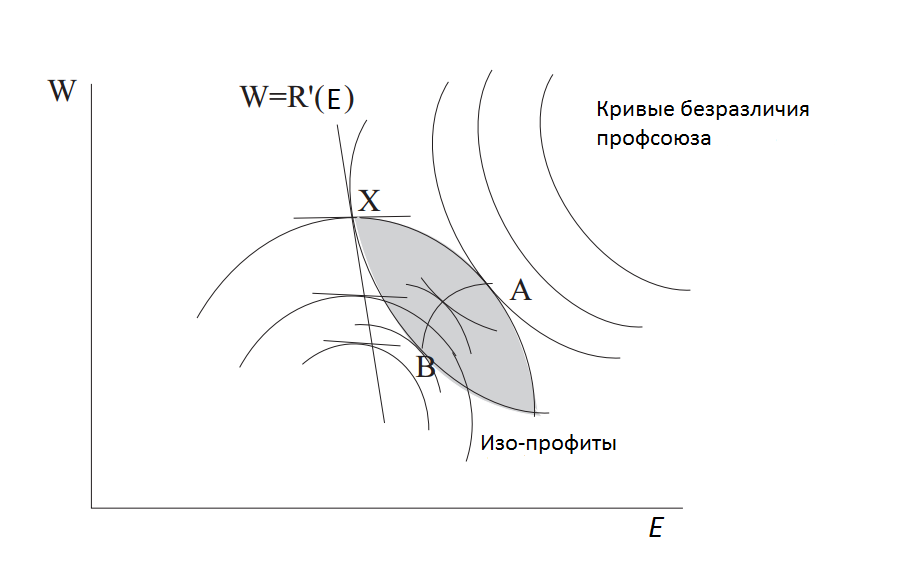
\includegraphics[width=1.0\linewidth]{monopoly_union.png}
	\caption{Криві байдужості гравців в моделі профспілка --- монополіст}
	\label{fig:monopoly_union}
\end{figure}

\subsection{Модель профспілка --- монополіст на тимчасових шкалах}
Ця модель в літературі не зустрічається і досліджена нами вперше.
У грі, так само як і в неперервнiй моделі, два гравця: профспілка $ P $ і фірма - монополіст
$ F $, чиїми важелями впливу на гру є $ W $ (заробітня плата робітника) і $ E $
(кількість найнятих робочих) відповідно. Кожен гравець вибирає одну з двох
стратегій: встановити низьке $ L $ або високе $ H $ значення керованого ним параметра.
У загальному вигляді гра може бути задана наступною матрицею виграшів:

\begin{table}[h]
	\centering
	\caption{}
		Матриця виграшів для моделі "профспілка --- монополіст"\\
		\normalsize
	\begin{tabular}{|l|l|l|l|}
		\hline
		\multicolumn{2}{|l|}{\multirow{2}{*}{}} & \multicolumn{2}{l|}{Профспілка} \\ \cline{3-4} 
		\multicolumn{2}{|l|}{}                  & $L$            & $H$            \\ \hline
		\multirow{2}{*}{Фірма}     & $L$     & $a,q$          & $b,v$          \\ \cline{2-4} 
		& $H$     & $c,x$          & $d,z$          \\ \hline
	\end{tabular}
	\label{tab:mono:prof}
\end{table}
Функцію корисності профспілки ми вважаємо лінійною: $U(W,E)=\lambda WE$, де $\lambda \in(0;1)$:
$$
	\frac{\partial U}{\partial W} > 0; 
	\quad 
	\frac{\partial U}{\partial E}~>~0 ; 
	\quad
	\frac{\partial^2 U}{\partial W^2} \leqslant 0
$$

$$
	U(0,E) = U(W,0) = U(0,0) = 0.
$$

Функція корисності фірми має вигляд $\Pi(W,E)=cP(\bar{K},E)-WE$:
$$P(\bar{K}, E)=A\bar{K}^\alpha E^\beta,$$ 
де $A$ --- коефіцієнт нейтрального технічного прогресу, $\alpha$ и $\beta$
---коефіцієнти еластичності валового внутрішнього продукту за капітальними і
трудовими затратами.

Для профспілки співвідношення між значеннями функції корисності для різних ігрових ситуацій
будуть наступними:
\begin{equation}
U(L,L) < U(L,H) \nsim U(H, L) < U(H,H).
\end{equation}
Співвідношення $U(L,H) \nsim U(H, L)$ не може бути визначено однозначно, так
як це <<політичний>> вибір між двома альтернативами: більша кількість
людей, які отримують меншу зарплатню (умовно <<лівий>> підхід до розподілу
доходів) або меншу кількість людей, які отримують велику зарплатню (умовно
<<правий>> підхід).

Для знаходження співвідношень між значеннями функції корисності фірми в різних ігрових ситуаціях
побудуємо графік~\ref{fig:monopoly_union1}.

\begin{figure}[h]
	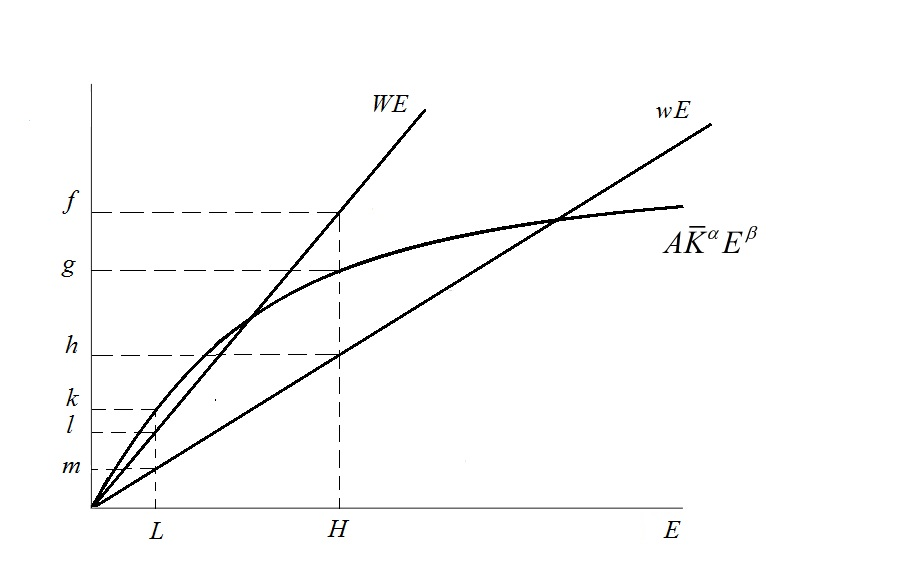
\includegraphics[width=1.0\linewidth]{monopoly_union2.jpg}
	\caption{Компоненти функції корисності фірми при різних рівнях заробітних плат}
	\label{fig:monopoly_union1}
\end{figure}

На малюнку $w$ --- низький рівень заробітних плат по стратегії $L$, $W$ --- виской рівень зарплат по стратегії $H$. 
Беручи до уваги, що за винятком кількості найнятих і рівня заробітних плат, всі інші величини постійні,
легко вивести наступне:
\begin{equation}
\Pi(H,H)=g-f < \Pi(H,L)=k-l < \Pi(L, L)=k-m < \Pi(L,H)=g-h.
\end{equation}

Отже матриця виграшів~(\ref{tab:mono:prof}) буде наступною:
\begin{table}[h]
	
	\centering
	\caption{}
	Матриця виграшів для моделі "профспілка --- монополіст"\\
		\normalsize

\begin{tabular}{|l|l|c|c|}
	\hline
	\multicolumn{2}{|l|}{\multirow{2}{*}{}} & \multicolumn{2}{l|}{Профспілка} \\ \cline{3-4} 
	\multicolumn{2}{|l|}{}                  & L                & H                \\ \hline
	\multirow{2}{*}{Фiрма}    & L   & a,q              & b,v              \\ \cline{2-4} 
	& H   & c,x              & d,z              \\ \hline
\end{tabular}
	\label{table:firm}
\end{table}\\
где $q < x \thickapprox v < z, 0 > d < b < a < c$.
